\documentclass[10pt,a4paper,oneside]{article}

% This first part of the file is called the PREAMBLE. It includes
% customizations and command definitions. The preamble is everything
% between \documentclass and \begin{document}.

\usepackage[margin=1in]{geometry}  % set the margins to 1in on all sides
\usepackage{graphicx}              % to include figures
\usepackage{amsmath}               % great math stuff
\usepackage{amsfonts}              % for blackboard bold, etc
\usepackage{amsthm}                % better theorem environments
\usepackage[english]{babel}
\usepackage[square, numbers]{natbib}
\usepackage[T1]{fontenc}
\usepackage[utf8]{inputenc}
\usepackage{lmodern}
\usepackage{amssymb}
\usepackage{authoraftertitle}
\usepackage{hyperref}
\usepackage{multicol}
\usepackage{caption}
\usepackage{subcaption}
\usepackage{placeins}
\usepackage{setspace}

%\onehalfspace
\singlespace

% Author
\author{Ondrej Škopek\\
Faculty of Mathematics and Physics\\
Charles University in Prague\\
\texttt{\href{mailto:oskopek@matfyz.cz}{oskopek@matfyz.cz}}}

\title{\textbf{DRAFT:} Individual software project -- specification -- CodeName:TEdit}

%\date{3. mája 2015}
\date{\today}

% hyperref

\hypersetup{
    bookmarks=true,         % show bookmarks bar?
    unicode=true,          % non-Latin characters in Acrobat’s bookmarks
    pdftoolbar=true,        % show Acrobat’s toolbar?
    pdfmenubar=true,        % show Acrobat’s menu?
    pdffitwindow=true,     % window fit to page when opened
    pdfstartview={FitV},    % fits the width of the page to the window
    pdftitle={\MyTitle},    % title
    pdfauthor={\MyAuthor},     % author
    pdfsubject={\MyTitle},   % subject of the document
    pdfcreator={\MyAuthor},   % creator of the document
    pdfproducer={\MyAuthor}, % producer of the document
    pdfkeywords={software} {project} {planning} {automated planning} {java} {javafx} {ipc} {transport domain}, % list of keywords
    pdfnewwindow=true,      % links in new PDF window
    colorlinks=false,       % false: boxed links; true: colored links
    linkcolor=red,          % color of internal links (change box color with linkbordercolor)
    citecolor=green,        % color of links to bibliography
    filecolor=magenta,      % color of file links
    urlcolor=cyan,           % color of external links
}


% various theorems, numbered by section

\newtheorem{thm}{Theorem}[section]
\newtheorem{lem}[thm]{Lemma}
\newtheorem{obsv}[thm]{Observation}
\newtheorem{cor}[thm]{Corollary}
\newtheorem{conj}[thm]{Conjecture}

\DeclareMathOperator{\id}{id}

\newcommand{\TODO}[1]{{\textbf{TODO:} #1}} % for TODOs
\newcommand{\comment}[1]{} % for comments

\newcommand{\dist}{\text{dist}} % distance function
\newcommand{\bd}[1]{\mathbf{#1}} % for bolding symbols 
\newcommand{\RR}{\mathbb{R}}      % for Real numbers
\newcommand{\ZZ}{\mathbb{Z}}      % for Integers
\newcommand{\col}[1]{\left[\begin{matrix} #1 \end{matrix} \right]}
\newcommand{\comb}[2]{\binom{#1^2 + #2^2}{#1+#2}}
\newcommand{\pname}{Codename:TEdit } % project name (or code name)

\begin{document}
\maketitle

\TODO Vymysliet nazov programu: TransportEditor, TEdit, VisualTransport











\section{Basic information}

\pname aims to be a problem editor and plan visualizer for the Transport domain from the International Planning Competition 2008.
The goal is to create an intuitive GUI desktop application for making quick changes and re-planning, but also designing a new problem dataset from scratch. \pname will help researchers working on this domain fine-tune their planners; they can visualize the various corner cases their planner fails to handle, step through the generated plan and find the points where their approach fails.

\subsection{The Transport planning domain}

Transport is a domain designed originally for the International Planning Competition (IPC, part of the International Conference on Automated Planning and Scheduling ICAPS).
Originally, Transport appeared at \href{http://icaps-conference.org/ipc2008/deterministic/Domains.html}{IPC-6 2008}.
Since then, it has been used in every IPC, specifically \href{http://www.plg.inf.uc3m.es/ipc2011-deterministic/}{IPC-7 2011}
and \href{https://helios.hud.ac.uk/scommv/IPC-14/}{IPC-8 2014}.

There are two basic formulations of the Transport domain family (i.e. two ``similar Transport domains''):
\begin{itemize}
\item \verb+transport-strips+ -- the classical, sequential Transport domain. See section \ref{transport-strips}.
\item \verb+transport-numeric+ -- the numerical Transport domain. See section \ref{transport-numeric}.
\end{itemize}

Both of these formulations have been used interchangeably in various competition tracks.
The following is an overview of the distinct datasets, their associated IPC competition, track at the competition and the formulation used (descriptions of the tracks in hyperlinks):

\begin{center}
\begin{tabular}{|c|c|c|c|}
\hline 
Dataset name & Competition & Track & Formulation \\ 
\hline 
netben-opt-6 & IPC-6 & \href{http://icaps-conference.org/ipc2008/deterministic/NetBenefitOptimization.html}{Net-benefit: optimal} & Numeric \\ 
\hline 
seq-opt-6 & IPC-6 & \href{http://icaps-conference.org/ipc2008/deterministic/SequentialSatisficing.html}{Sequential: satisficing} & STRIPS \\ 
\hline 
seq-sat-6 & IPC-6 & \href{http://icaps-conference.org/ipc2008/deterministic/SequentialOptimization.html}{Sequential: optimal} & STRIPS \\ 
\hline 
tempo-sat-6 & IPC-6 & \href{http://icaps-conference.org/ipc2008/deterministic/TemporalSatisficing.html}{Temporal: satisficing} & Numeric \\ 
\hline 
seq-agl-8 & IPC-8 & \href{https://helios.hud.ac.uk/scommv/IPC-14/seqagi.html}{Sequential: agile} & STRIPS \\ 
\hline 
seq-mco-8 & IPC-8 & \href{https://helios.hud.ac.uk/scommv/IPC-14/seqmulti.html}{Sequential: multi-core} & STRIPS \\ 
\hline 
seq-opt-8 & IPC-8 & \href{https://helios.hud.ac.uk/scommv/IPC-14/seqopt.html}{Sequential: optimal} & STRIPS \\ 
\hline 
seq-sat-8 & IPC-8 & \href{https://helios.hud.ac.uk/scommv/IPC-14/seqsat.html}{Sequential: satisficing} & STRIPS \\ 
\hline 
\end{tabular} 
\end{center}

Short descriptions of the various tracks and subtracks can be found in the rule pages of
\href{https://helios.hud.ac.uk/scommv/IPC-14/rules.html}{IPC-6}
and the  \href{http://icaps-conference.org/ipc2008/deterministic/CompetitionRules.html}{rule page of IPC-8}.

Unfortunately, we weren't able to acquire the datasets for IPC-7, as the Subversion repository that promises to contain them is unavailable (\url{http://www.plg.inf.uc3m.es/ipc2011-deterministic/Domains.html}).

% Comparison with Trucks from IPC-5
%In general, the Transport domain family is very similar to the Trucks domain family from \href{http://idm-lab.org/wiki/icaps/ipc2006/deterministic/}{IPC-5 2006}. The key differences are ...

\subsection{Transport STRIPS formulation description}\label{transport-strips}

The STRIPS version of Transport is a logistics domain -- vehicles with limited capacities drive around on a (generally asymmetric) positively-weighted oriented graph, picking up and dropping packages along the way. Picking up or dropping a package costs 1, driving along a road costs depending on the edge weight. All packages have a size of 1. The general aim is to minimize the total cost, while delivering all packages to their destination.

\subsection{Transport Numeric formulation description}\label{transport-numeric}

The numerical version of Transport is very similar to the STRIPS version, see section \ref{transport-strips}. The key differences are:
\begin{itemize}
\item Package sizes can now be any positive number.
\item The concept of fuel -- every vehicle has a maximum fuel level, current fuel level, and all roads have a fuel demand (generally different than the length of the road). A vehicle can refuel if there is a petrol station at the given location. Refuelling always fills the vehicle's tank to the max.
\item The introduction of time:
\begin{itemize}
\item The duration of driving along a road is equal to it's length.
\item The duration of picking a package up or dropping it off is equal to 1.
\item The duration of refuelling is equal to 10.
\item A vehicle cannot pick up or drop packages concurrently -- it always handles packages one at a time.
\item A vehicle cannot do other actions during driving to another location (it is essentially placed ``off the graph'' for the duration of driving).
\end{itemize}
\item The cost function is removed (we now minimize the total duration of a plan).
\end{itemize}


















\section{Feature requirements}

In this section, we present the basic functionality requirements for \pname.

\subsection{Functionality overview}

The basic work flow of \pname consists of the following user's steps:
\begin{itemize}
\item Select which formulation of the Transport domain they want to work with.
\item Load a problem of the given domain. See section \ref{inputoutput} for details on the input format.
\item \pname draws the given graph as good as it can.
\item Iterate among the following options:
\begin{itemize}
\item Load a planner executable and let \pname run the planner on the loaded problem instance.
\item Step through the individual plan actions and let \pname visualize them.
\item Edit the graph: add/remove/edit the location or properties of vehicles, packages, roads, locations and possibly petrol stations.
\item Save the currently generated plan.
\item Save the problem (along with the graph drawing hints). For details, see section \ref{inputoutput}.
\end{itemize}
\item Save and close the currently loaded problem. Exit the application, or go back to the first step.
\end{itemize}

There are a lot of requirements that arise from the typical work flow above. We will describe them in the next few sections.

\subsection{User interface functionality}

In order for \pname to be useful to it's users, it has to have enable a quick and efficient work flow.
The biggest challenge will be to design an intuitive and responsive graphical user interface.
Key parts of the user interface are:
\begin{itemize}
\item A large and not crowded drawing of the road graph, showing only the most relevant information, possibly letting the user display details on-demand.
\item A clear and concise list of actions in the plan the user wants to visualize.
\item A panel of tools to edit the problem and graph with.
\end{itemize}

We will describe these three in detail in the following sections.

\subsubsection{Graph visualization}

Above all, the graph should be reasonably well arranged and drawn. However, drawing an arbitrary graph is considered a hard problem on it's own. \TODO citation needed
We will focus on implementing a reasonable graph drawing algorithm and let the user make manual drag-and-drop style changes on top of the graph drawing we produce.

A more specific property of the Transport domain graphs is that they have quite a lot of data on the edges (roads) and vertexes (locations) -- road lengths, fuel demands, location names and petrol station, package and vehicle current locations.
Clearly, this cannot fit on the graph drawing at once -- we will have to do selective drawing of the information in order
not to crowd the graph.
Popping up overlays on user mouse-over
or a graph legend where the user can select what info to currently show are just a few options.

\subsubsection{Plan action list}

\TODO Step-through the plan, step-back the plan (scroll? fluent?)

\subsubsection{Editing tools}

A big feature of \pname is editing the domain problems on the fly. 

\subsection{Performance}
\subsection{Extensibility}

\subsection{Bonus features} \TODO ?
\TODO Verify plans? VAL









\section{Program decomposition}

\subsection{Modules}
\TODO separate RP and BP
\subsection{UML diagram}








\section{Software description}


\subsection{Analysis}

\TODO To offer the functionality, ... + show ideas that weren't used.

\FloatBarrier
\begin{figure}
        \centering
        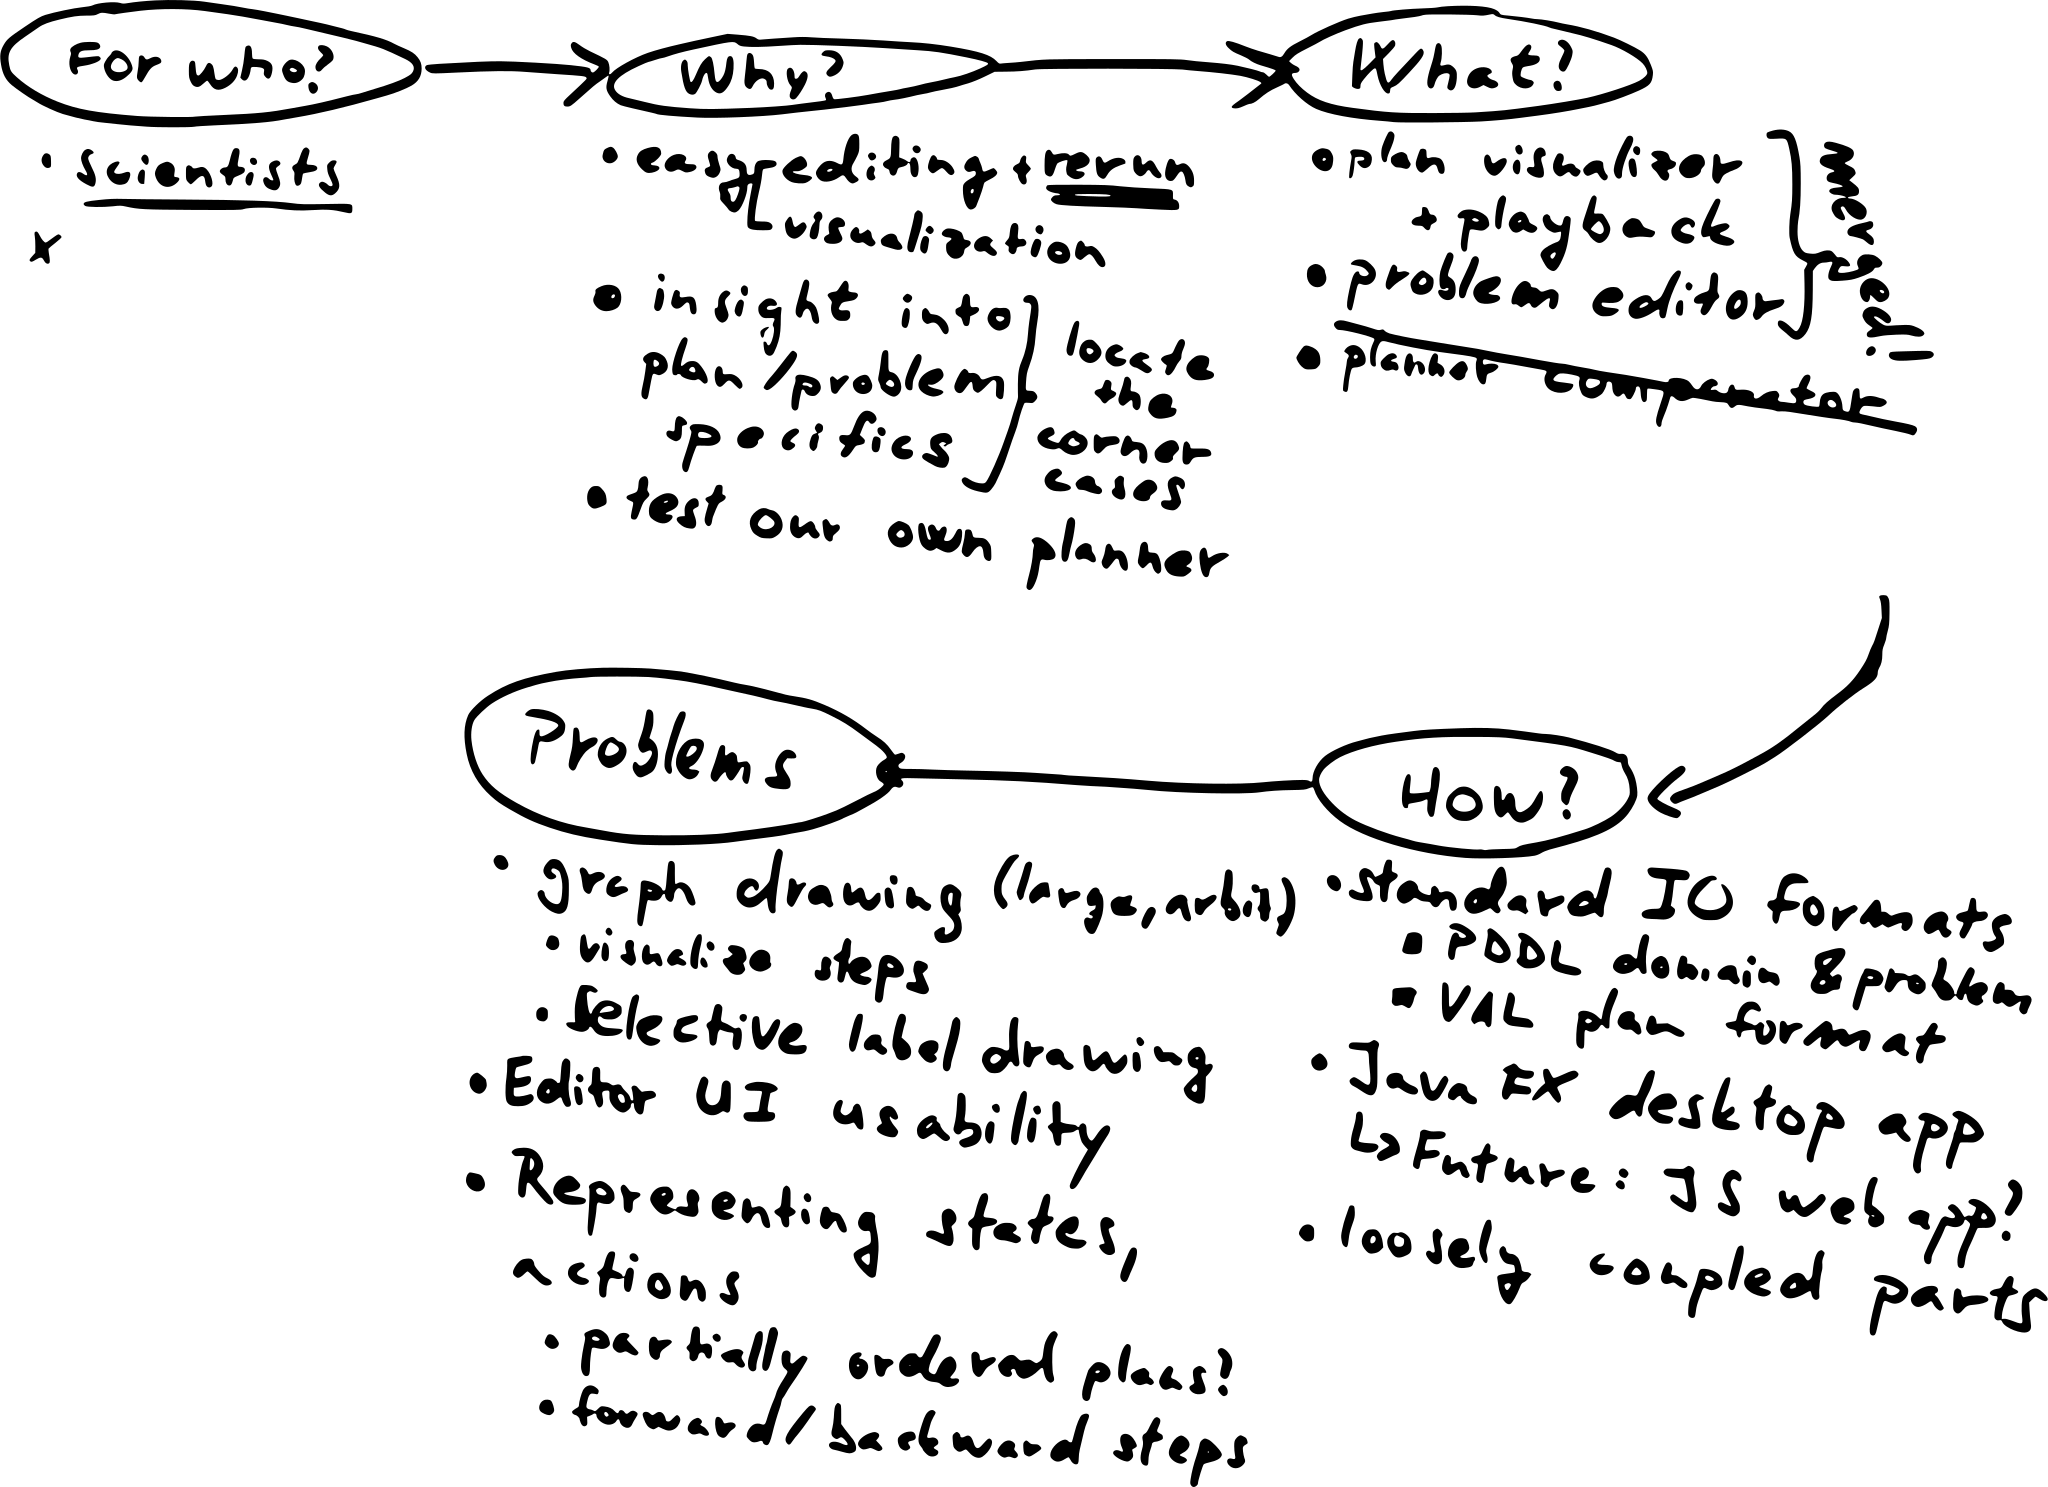
\includegraphics[width=0.8\textwidth]{../data/img/pdf/spec}
        \caption{Mindmap}
        \label{fig:mindmap}
\end{figure}
\FloatBarrier

\TODO Should be modular / extensible



\subsection{Used technologies}
\subsubsection{Environment dependencies}
\subsection{Technological problems and their proposed solutions}
\TODO FXML communication -- Weld(CDI)


\subsection{User and developer documentation}









\section{Input \& output format} \label{inputoutput}


\TODO an extension to the input PDDL in comments ;coordinates










\section{User interface}


\subsection{Main screen}

\FloatBarrier
\begin{figure}
        \centering
        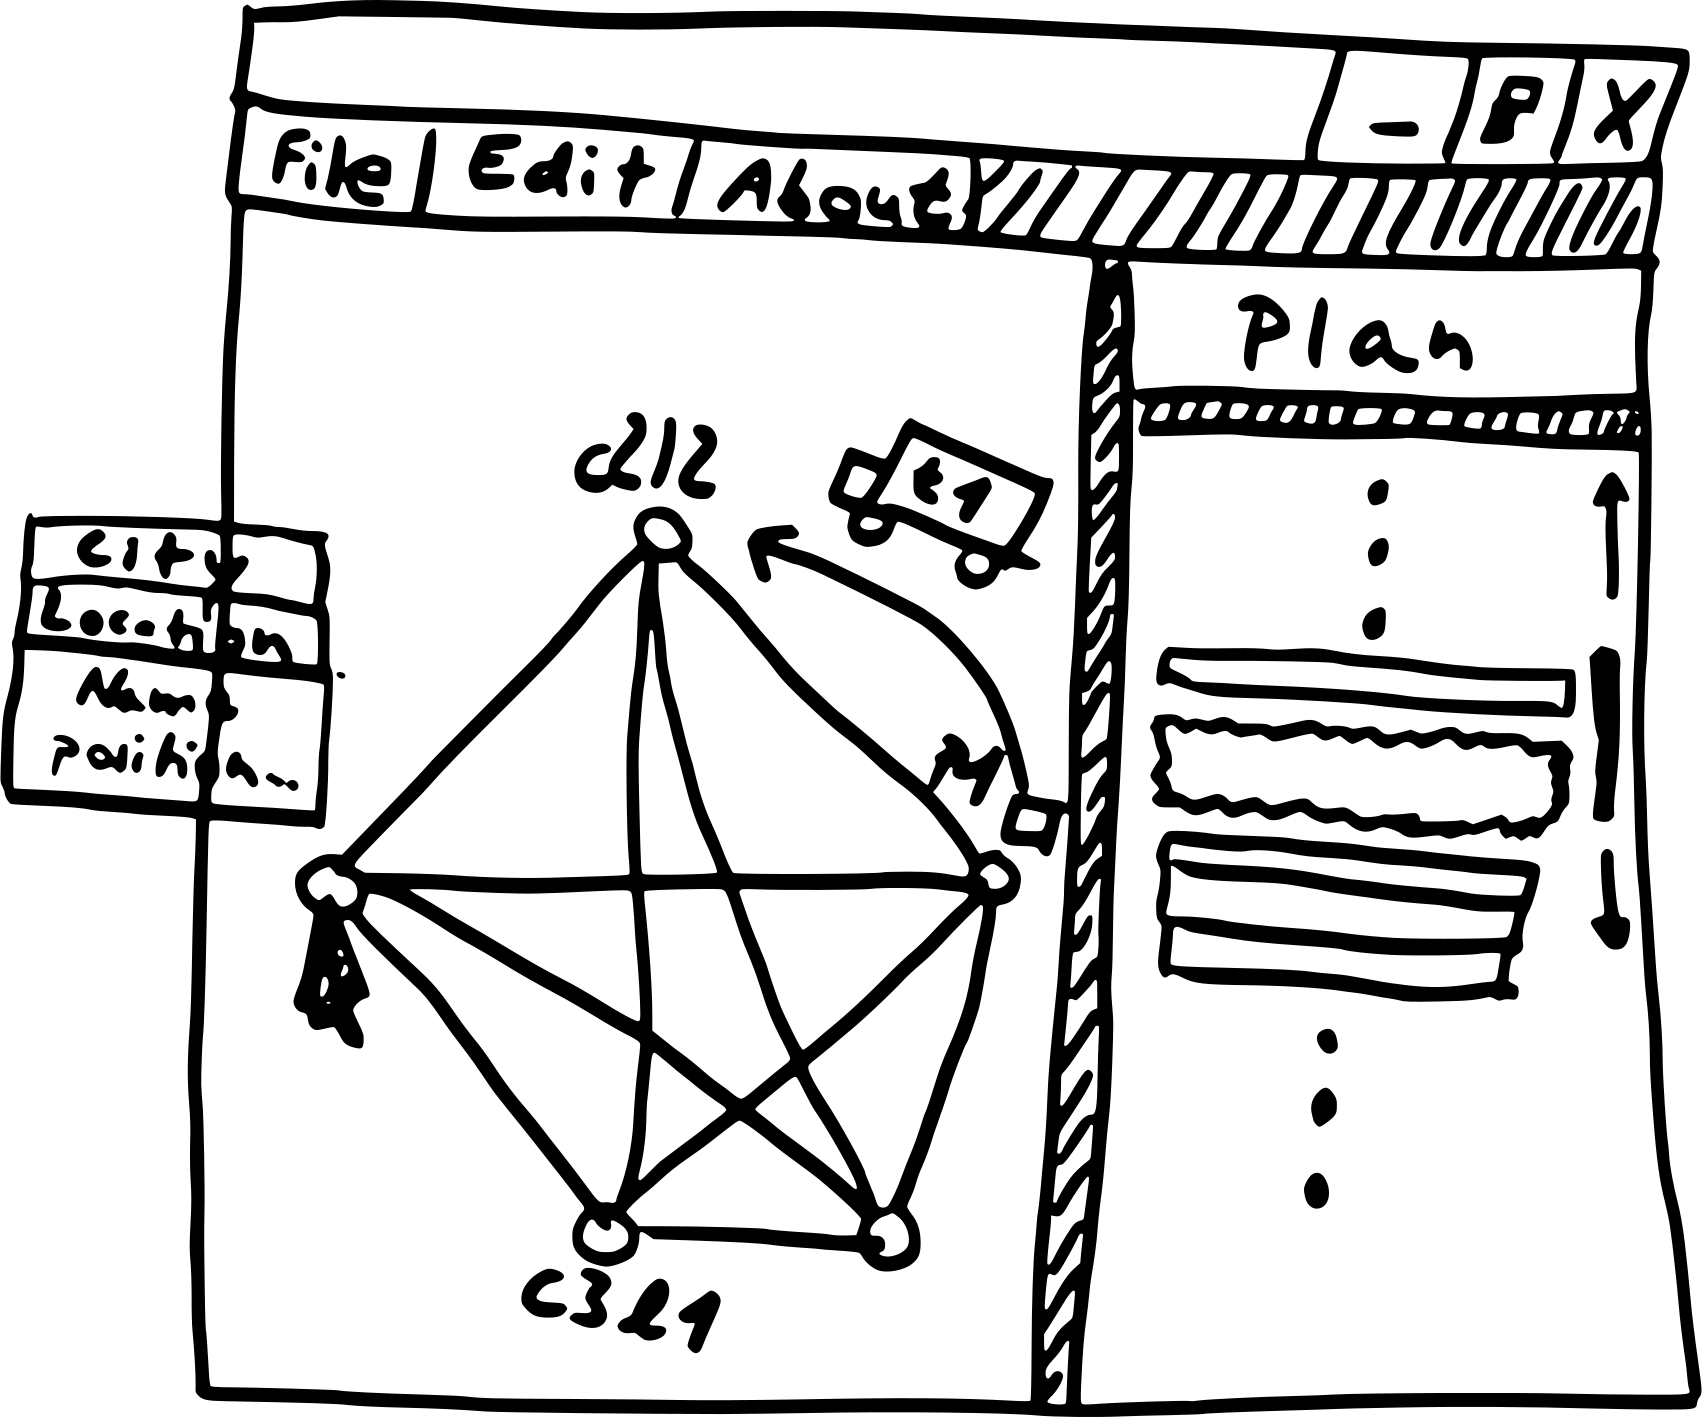
\includegraphics[width=0.8\textwidth]{../data/img/pdf/gui}
        \caption{Abstract GUI prototype}
        \label{fig:gui}
\end{figure}
\FloatBarrier

\TODO Need to do selective label drawing (too crowded) with popup info boxes
\TODO Make the graph nodes moveable
\TODO scrollable own widget (transparent, fluid) for the plan. --> partial order plans? No.
\TODO How do we simulate movement on an abstract graph?

\subsection{Helper screens}















\section{Open questions and ending notes}

\begin{itemize}
    \item Do we support the numerical Transport domain too?
    \item Is it safe to assume that symmetric edges are weight-symmetric? (all datasets have this) -- more of a planner question
\end{itemize}

The conversion from hand-drawn pictures to vector images was done using the wonderful
open-source project cartoonist: \url{https://github.com/honzajavorek/cartoonist}.

{
\footnotesize % 10pt in 12pt article size
%%% Bibliography (literature used as a source)
%%%
%%% We employ bibTeX to construct the bibliography. It processes
%%% citations in the text (e.g., the \cite{...} macro) and looks up
%%% relevant entries in the bibliography.bib file.
%%%
%%% The \bibliographystyle command selects, which style will be used
%%% for references from the text. The argument in curly brackets is
%%% the name of the corresponding style file (*.bst). Both styles
%%% mentioned in this template are included in LaTeX distributions.

%\bibliographystyle{plainnat}    %% Author (year)
\bibliographystyle{unsrt}     %% [number]

\renewcommand{\bibname}{Bibliography}

%%% Generate the bibliography. Beware that if you cited no works,
%%% the empty list will be omitted completely.

\bibliography{bibliography}

%%% If case you prefer to write the bibliography manually (without bibTeX),
%%% you can use the following. Please follow the ISO 690 standard and
%%% citation conventions of your field of research.

% \begin{thebibliography}{99}
%
% \bibitem{lamport94}
%   {\sc Lamport,} Leslie.
%   \emph{\LaTeX: A Document Preparation System}.
%   2nd edition.
%   Massachusetts: Addison Wesley, 1994.
%   ISBN 0-201-52983-1.
%
% \end{thebibliography}

}
\end{document}